\documentclass[runningheads]{llncs}
\usepackage[utf8]{inputenc}
\usepackage[english]{babel}
\usepackage[T1]{fontenc}
\usepackage{graphicx}
\usepackage{amsmath}
\usepackage{amssymb}
\usepackage{url}
\usepackage{cite}
\usepackage{tabularx}
\usepackage{rotating}
\title{Learning-Enhanced Security-Constrained\\ Unit Commitment Problem}


\author{Egor Grishin\inst{1}}
\authorrunning{E. Grishin}

\institute{Skoltech, Moscow, Russia}

\begin{document}
\maketitle

\begin{abstract}
The Security-Constrained Unit Commitment (SCUC) problem determines day-ahead generator schedules while enforcing N-1 security constraints under a DC power-flow approximation. This paper compares k-nearest-neighbor warm starts, branching hints, post-contingency screening, graph-based screening, and lazy N-1 enforcement. These methods represent widely used solver-native, data-driven, and learning-guided acceleration families. Tests across the main six MATPOWER cases (14 to 300 buses) show that the dominant gains come from reducing or delaying post-contingency constraints: the best configuration reaches up to 25.8x speedup on case89pegase and 9.6x on average, while warm starts and hints provide smaller secondary gains (around 1.1x). An additional case1354pegase stress test checks whether the lazy design runs on a much larger grid.
\keywords{Hybrid approach \and Large-scale problem \and Machine learning \and Mixed-integer linear programming \and Unit commitment.}
\end{abstract}


\section{Introduction}
We tackle the Security-Constrained Unit Commitment (SCUC) problem, determining which generators run at what capacity over a day-ahead horizon while keeping costs low and the grid stable. In the main benchmark, this horizon has 24 hourly periods. The large scalability stress test uses 36 periods. SCUC sits at the core of day-ahead electricity markets, where solutions must be found quickly and reliably.

The computational difficulties come from two sources. First, thermal generators have minimum runtime requirements and cannot change output arbitrarily fast between hours. These temporal constraints tie decisions across all time periods, preventing simple hour-by-hour optimization. Second, we enforce N-1 security: the grid must survive any single component failure (transmission line or generator). For each hour, hundreds or thousands of contingency scenarios must be checked explicitly. With transmission lines numbering in the hundreds, these constraints grow quadratically, creating computational bottlenecks for real-world grids.

Fully explicit N-1 MILP formulations can become difficult for general-purpose solvers under tight operational time limits. Adding renewable energy's variability makes the problem worse. Even state-of-the-art algorithms may hit time limits before proving high-quality solutions for large grids, a critical issue when markets clear on strict schedules. We need acceleration methods that maintain solution quality while significantly reducing solve time.

The formulations for the SCUC problem have evolved significantly, transitioning from early heuristics~\cite{Merlin1983} to the more sophisticated and computationally efficient modern MILP models. A computationally efficient MILP formulation for thermal unit commitment with piecewise-linear costs was introduced in~\cite{Carrion2006}. More accurate formulations for complex unit dynamics have since been developed~\cite{Ostrowski2012}. Decomposition methods such as Benders' decomposition and Lagrangian relaxation are often used to separate the main commitment problem from the power grid and security subproblems~\cite{Morales2013}.


On the power grid modeling side, the DC power flow approximation is the standard for SCUC due to its linearity and scalability. Power Transfer Distribution Factors (PTDFs) are widely used to model base-case flows, while Line Outage Distribution Factors (LODFs) provide an efficient way to approximate post-contingency flows without solving the power flow problem for each contingency~\cite{Christie2000, Tejada2018}.

To manage the quadratic growth of contingency constraints, a dynamic constraint generation technique is often adopted~\cite{Tejada2018}.
In this approach, a subset of potential binding constraints is initially included, and additional constraints can be added as necessary during the branching process~\cite{Tejada2018}. A complementary approach involves screening techniques that aim to discard redundant contingencies in advance using power grid sensitivities or historical data~\cite{Holzer2024}.

Machine learning has become a major tool for accelerating combinatorial optimization~\cite{Bengio2021}. In power-system optimization, related work includes learned active-set and warm-start strategies for large-scale SCUC~\cite{Xavier2019}, cone-programming relaxations for SCUC under uncertainty~\cite{Quarm2021}, feasibility-aware neural approximations for constrained optimization and optimal power flow~\cite{Donti2021}, and machine-learning warm starts for constraint generation in MILP~\cite{JimenezCordero2022}. Xavier~\textit{et al.}~\cite{Xavier2019} report SCUC solves that are on average $4.3\times$ faster with optimality guarantees and $10.2\times$ faster without optimality guarantees, on test systems up to 6{,}515 buses and 1{,}388 units. Jim{\'e}nez-Cordero \textit{et al.}~\cite{JimenezCordero2022} report roughly $2$--$10\times$ on MIPLIB-style instances for warm-starting constraint generation. Wrong ML predictions, on the other hand, could produce an insecure schedule.

Our contribution is a controlled empirical study of ML acceleration inside a MILP SCUC workflow. The ML components propose starts, branching priorities, screening decisions, or lazy-cut budgets. Final schedules are checked by a full N-1 audit. We test warm starts, branching guidance, constraint screening, and lazy enforcement both individually and combined. The grid is modeled using the DC approximation. Base-case flows use PTDFs. Post-contingency flows use LODFs. This gives a linear and scalable representation of grid dynamics. Our best average speedup is $9.64\times$ for the recommended 1-NN screening setting. The best lazy-callback variant reaches $8.61\times$. These gains are in the same order of magnitude as the prior ML-accelerated SCUC work cited above. Feasibility is claimed only after the full audit, not from the predictor itself.

\section{Model Definition}

A deterministic SCUC is solved over time periods $\mathcal{T}$ for generators $\mathcal{G}$, buses $\mathcal{B}$, transmission lines $\mathcal{L}$, and reserve products $\mathcal{R}$. Indices $g,b,\ell,k,t,s$ refer to generators, buses, lines, reserve products, time periods, and cost segments, respectively. Variables are commitment $u_{g,t}$, startup/shutdown $v_{g,t},w_{g,t}$, segment output $p^{\mathrm{seg}}_{g,t,s}$, total generation $p_{g,t}=u_{g,t}\underline{P}_{g,t}+\sum_s p^{\mathrm{seg}}_{g,t,s}$, reserves $r_{k,g,t}$, reserve shortfall $h_{k,t}$, base flow $f_{\ell,t}$, base overflow slacks $\overline{o}_{\ell,t},\underline{o}_{\ell,t}$, and shared N-1 slacks $\overline{c}_{\ell,t},\underline{c}_{\ell,t}$. The binary domains are $u_{g,t},v_{g,t},w_{g,t}\in\{0,1\}$; generation segments, reserves, reserve shortfalls, and slacks are non-negative.

The parameters $\underline{P}_{g,t}$ and $\overline{P}_{g,t}$ are minimum and maximum generator outputs, $\mathcal{K}_g$ is the set of cost segments of generator $g$, $A_{g,s,t}$ is segment capacity, $D_{b,t}$ is demand, and $R_{k,t}$ is reserve requirement. Ramp and startup/shutdown limits are denoted by $RU_g,RD_g,SU_g,SD_g$, while $U_g$ and $D_g$ are minimum up- and down-times. The subscripts distinguish demand $D_{b,t}$ from minimum down-time $D_g$. Thermal logic is:
\begin{equation}
0\le p^{\mathrm{seg}}_{g,t,s} \le A_{g,s,t}\,u_{g,t}, \ \forall g,t,s. \label{eq:seg-link}
\end{equation}
\begin{equation}
\sum_{g}\Big(u_{g,t}\underline{P}_{g,t}+\sum_{s\in \mathcal{K}_g}p^{\mathrm{seg}}_{g,t,s}\Big)=\sum_{b}D_{b,t}, \ \forall t. \label{eq:balance}
\end{equation}
\begin{equation}
\sum_{s\in \mathcal{K}_g}p^{\mathrm{seg}}_{g,t,s}+\sum_{k}r_{k,g,t}\le (\overline{P}_{g,t}-\underline{P}_{g,t})u_{g,t}, \ \forall g,t. \label{eq:res-head}
\end{equation}
\begin{equation}
\sum_{g}r_{k,g,t} + h_{k,t} \ge R_{k,t}, \ \forall k,t. \label{eq:res-req}
\end{equation}
\begin{align}
u_{g,t}-u_{g,t-1} &= v_{g,t}-w_{g,t}, \label{eq:su-def}\\
v_{g,t}+w_{g,t} &\le 1. \label{eq:su-excl}
\end{align}
\begin{align}
p_{g,t}-p_{g,t-1} &\le RU_g\,u_{g,t-1} + SU_g\,v_{g,t}, \label{eq:ramp-up}\\
p_{g,t-1}-p_{g,t} &\le RD_g\,u_{g,t} + SD_g\,w_{g,t}. \label{eq:ramp-dn}
\end{align}
\begin{align}
\sum_{\tau=t-U_g+1}^{t} v_{g,\tau} \le u_{g,t}, \quad
\sum_{\tau=t-D_g+1}^{t} w_{g,\tau} \le 1-u_{g,t}. \label{eq:min-ud}
\end{align}
Early periods use the initial commitment and residual up/down times from the instance data.

\begin{equation}
\mathrm{inj}_{b,t}=\sum_{g\in\mathcal{G}_b} p_{g,t} - D_{b,t},
\end{equation}
where $\mathcal{G}_b$ is the generator set at bus $b$. Base-case flow uses the power transfer distribution factor $\mathrm{PTDF}_{\ell,b}$:
\begin{equation}
f_{\ell,t}=\sum_{b\neq b^{\mathrm{ref}}}\mathrm{PTDF}_{\ell,b}\,\mathrm{inj}_{b,t},
\label{eq:flow-def}
\end{equation}
where $b^{\mathrm{ref}}$ is the reference bus. Normal and emergency line ratings are denoted by $F^{\mathrm{N}}_{\ell,t}$ and $F^{\mathrm{E}}_{\ell,t}$. Normal line limits are:
\begin{equation}
-F^{\mathrm{N}}_{\ell,t}-\underline{o}_{\ell,t} \ \le\ f_{\ell,t}\ \le\ F^{\mathrm{N}}_{\ell,t}+\overline{o}_{\ell,t}
\label{eq:base-lims}
\end{equation}
For line outage $m$, the line outage distribution factor $\mathrm{LODF}_{\ell,m}$ gives
\begin{equation}
f_{\ell,t}^{m} \approx f_{\ell,t}+\mathrm{LODF}_{\ell,m}f_{m,t}. \label{eq:lodf}
\end{equation}
The corresponding emergency limits are
\begin{equation}
-F^{\mathrm{E}}_{\ell,t}-\underline{c}_{\ell,t}\ \le\ f_{\ell,t}+\mathrm{LODF}_{\ell,m}f_{m,t}\ \le\ F^{\mathrm{E}}_{\ell,t}+\overline{c}_{\ell,t}.
\label{eq:cont-line}
\end{equation}
For generator outage $g$ at bus $b(g)$:
\begin{equation}
-F^{\mathrm{E}}_{\ell,t}-\underline{c}_{\ell,t}\ \le\ f_{\ell,t}-\mathrm{PTDF}_{\ell,b(g)}\,p_{g,t}\ \le\ F^{\mathrm{E}}_{\ell,t}+\overline{c}_{\ell,t}.
\label{eq:cont-gen}
\end{equation}
This expression assumes reference-bus balancing of the lost generator output; distributed balancing would require participation-factor terms.

\begin{align}
\min \ \ & \sum_{t}\sum_{g}\Big( C^{\min}_{g,t}\,u_{g,t} + \sum_{s\in\mathcal{K}_g} C^{\mathrm{seg}}_{g,s,t}\, p^{\mathrm{seg}}_{g,t,s} \Big) \nonumber\\
& + \sum_{t}\sum_{g} C^{\mathrm{su}}_g\, v_{g,t} \label{eq:obj}\\
& + \sum_{t}\sum_{k\in\mathcal{R}} \pi^{\mathrm{res}}_k\, h_{k,t} \nonumber\\
& + \sum_{t}\sum_{\ell\in\mathcal{L}} \pi^{\mathrm{flow}}_{\ell,t}(\overline{o}_{\ell,t}+\underline{o}_{\ell,t}) \nonumber\\
& + \gamma \sum_{t}\sum_{\ell\in\mathcal{L}} \pi^{\mathrm{flow}}_{\ell,t}(\overline{c}_{\ell,t}+\underline{c}_{\ell,t}). \nonumber
\end{align}
The coefficients $C^{\min}_{g,t}$, $C^{\mathrm{seg}}_{g,s,t}$, and $C^{\mathrm{su}}_g$ are no-load, segment-production, and startup costs. The penalties $\pi^{\mathrm{res}}_k$ and $\pi^{\mathrm{flow}}_{\ell,t}$ price reserve shortfalls and transmission overflows. The factor $\gamma>1$ gives post-contingency slacks a larger penalty than base-case slacks. Since overflow slacks can make the optimization model formally feasible despite physical violations, N-1 feasibility is determined only by the post-solve audit with zero raw violations.

\section{Acceleration Framework}
We compare four acceleration mechanisms: screening, lazy enforcement, warm starts, and branching guidance. They affect different parts of the MILP process. Screening changes the initial constraint set, lazy enforcement delays constraints until they are violated, warm starts provide primal information, and branching guidance changes the solver's search priorities.

The common design principle is to use learning only as guidance inside a solver-checked workflow. None of the methods replaces the MILP objective or the post-solve feasibility audit. This is important for SCUC because an incorrect prediction can be useful if it only changes the order in which constraints or branches are explored, but it is unacceptable if it silently removes a security requirement from the final schedule. For this reason, the acceleration methods are evaluated not only by runtime but also by whether the audited solution satisfies the full N-1 constraint set.

\paragraph{Constraint Screening (PRUNE-$\tau$).}
PRUNE-$\tau$ is a 1-nearest-neighbor screener using z-scored load shape and level statistics. Here $T=|\mathcal{T}|$, $L_t=\sum_b D_{b,t}$ is total load, and $\mu_L,\sigma_L$ are its sample mean and standard deviation:
\begin{equation}
z_t=\frac{L_t-\mu_L}{\sigma_L}, \ \mu_L=\frac{1}{T}\sum_t L_t, \ \sigma_L^2=\frac{1}{T-1}\sum_t(L_t-\mu_L)^2.
\end{equation}
The feature vector is
\begin{equation}
\phi=\big[z_0,\dots,z_{T-1},\ \mu_L,\ \max_t L_t,\ \sum_t L_t,\ \sigma_L\big].
\end{equation}
The level-sensitive entries avoid a degeneracy of pure z-scoring. Uniformly shifted load profiles would otherwise look identical. The peak load $\max_t L_t$ captures the maximum stress level. It is not determined by the mean load and is relevant for commitment and congestion patterns. Since $T$ is fixed across instances, $\sum_t L_t=T\mu_L$ does not add an independent descriptor. We retain it to give extra weight to the average load level in the nearest-neighbor metric. This matches the feature representation used in the experiments. For a target instance, $\phi^{(i)}$ denotes a historical feature vector, and the nearest solved dispatch $\hat{\imath}=\arg\min_i \|\phi-\phi^{(i)}\|_2$ estimates post-contingency flows. We use
$p^{(\hat{\imath})}_{g,t}$ as
$
p^{\mathrm{pred}}_{g,t} := p^{(\hat{\imath})}_{g,t},
$ and combine it with target demand $D_{b,t}$ to form predicted injections:
\begin{equation}
\mathrm{inj}^{\mathrm{pred}}_{b,t}=\sum_{g\in\mathcal{G}_b} p^{\mathrm{pred}}_{g,t} - D_{b,t}.
\end{equation}

The minimum emergency margin for line-outage pair $(\ell,m)$ is then computed from the predicted base flows $f^{\mathrm{pred}}_{\ell,t}$ and outage-line flows $f^{\mathrm{pred}}_{m,t}$:
\begin{equation}
s^{m}_{\ell}=\min_t \frac{F^{\mathrm{E}}_{\ell,t}-|f^{\mathrm{pred}}_{\ell,t}+\mathrm{LODF}_{\ell,m}f^{\mathrm{pred}}_{m,t}|}{F^{\mathrm{E}}_{\ell,t}}.
\end{equation}
Generator-outage pairs use the analogous margin $s^g_\ell$ from Eq.~\eqref{eq:cont-gen}, replacing the post-contingency expression by $f^{\mathrm{pred}}_{\ell,t}-\mathrm{PTDF}_{\ell,b(g)}p^{\mathrm{pred}}_{g,t}$. Pairs whose corresponding margin is at least $\tau$ are pruned for all time periods. Thus $\tau$ controls conservatism: smaller values prune more contingency pairs, whereas larger values retain more post-contingency constraints.

This screening rule is deliberately simple. It does not attempt to learn the complete unit-commitment map, and it does not require a neural architecture or end-to-end differentiability through the solver. Instead, it uses historical solved dispatches as local prototypes for likely power-flow patterns. The advantage is that it is cheap to train and transparent to inspect: a retained or removed pair can be traced to the predicted emergency margin. The disadvantage is that it can fail when a new load profile is close in feature space but has a different congestion pattern, which motivates the strict audit and the comparison with lazy enforcement.

In the experiments, PRUNE is used as a static pre-solve reduction. Once a constraint is removed, it is not reintroduced by this screening rule alone. Therefore thresholds are selected by audited feasibility, not only by speed. The more aggressive thresholds are useful as ablations because they reveal how much of the speedup comes from model-size reduction and how quickly feasibility can deteriorate when the reduced model becomes too optimistic.

\paragraph{Constraint Screening (GNN).}

The GNN scores critical lines on a line graph: nodes are transmission lines, and edges connect lines sharing a bus. Features include susceptance, average limits, and endpoint loads. The binary label $y_\ell$ marks whether line $\ell$ is critical. The threshold $y_{\mathrm{thr}}$ is the historical loading threshold:
\begin{equation}
y_\ell= 1\ \iff\ \max_t \frac{|f_{\ell,t}|}{F^{\mathrm{E}}_{\ell,t}} \ge y_{\mathrm{thr}},\ y_{\mathrm{thr}}=0.70.
\end{equation}

A two-layer GraphSAGE classifier~\cite{Hamilton2017} predicts the criticality probability $\hat p_\ell\in[0,1]$. With inference threshold $\theta=0.60$:
\begin{align}
\text{line outage } m:\quad &\text{keep }(\ell,m)\iff (\hat p_\ell\ge\theta)\ \text{or}\ (\hat p_m\ge\theta),\\
\text{gen outage } g:\quad  &\text{keep }(\ell,g)\iff \hat p_\ell\ge\theta.
\end{align}
The model uses hidden size 64 and Adam with learning rate $10^{-3}$. On case300, it reaches precision 0.83, recall 0.51, and F1 0.63. Sec.~\ref{sec:experiments} shows no consistent runtime gain over 1-NN.

The GNN is included to test whether topology-aware features can improve screening beyond nearest-neighbor load matching. Its line-graph representation lets information pass between adjacent transmission elements, which is natural for cascading congestion patterns. However, the supervised labels are sparse on small cases, because only a small fraction of lines approach emergency limits in the historical solutions. This makes the classifier difficult to train robustly outside the larger cases. The downstream question is therefore empirical: even if the GNN identifies critical lines reasonably well, the reduced MILP may not become easier than the 1-NN version if both methods retain nearly the same important constraints.

\paragraph{Lazy Enforcement (LAZY, BANDIT).}
LAZY enforces post-contingency constraints through callbacks with Gurobi's \texttt{LazyConstraints=1} parameter enabled~\cite{GurobiLazy}. The callback checks integer incumbents. If $f^{m}_{\ell,t}$ violates $F^{\mathrm{E}}_{\ell,t}$, inequalities of the form~\eqref{eq:cont-line} are added as lazy constraints. 

The full LAZY variant adds all detected line- and generator-outage violations, so any accepted incumbent has passed the same N-1 check used in the post-solve audit. Fixed-$K$ adds only the top-$K$ violations per callback, reducing callback overhead but allowing small residual violations if the search stops early. BANDIT chooses $K$ from the cut-budget set $\mathcal{K}^{\mathrm{cut}}=\{64,128,256\}$ with reward $R_t=-N_t^{\mathrm{added}}$, where $t$ is the callback counter in this paragraph and $N_t^{\mathrm{added}}$ is the number of cuts added at that callback. The exploration rate is $\varepsilon=0.1$, and $\bar R_K$ is the empirical mean reward for budget $K$:
\begin{equation}
K_{t+1}=\begin{cases}
\text{uniformly from }\mathcal{K}^{\mathrm{cut}}, & \text{with probability }\varepsilon, \\
\arg\max_{K\in\mathcal{K}^{\mathrm{cut}}}\bar{R}_K, & \text{with probability }1-\varepsilon.
\end{cases}
\end{equation}
All variants use the solver callback API.

Lazy enforcement changes the timing of constraint generation rather than the definition of feasibility. The initial model contains the base commitment, dispatch, and normal-flow constraints, while the callback checks incumbent solutions against post-contingency limits. If a violated contingency is found, the incumbent is rejected and the corresponding linear cut is added. This can be much faster than building the full static N-1 model because many contingency constraints never become active along the solver trajectory. The trade-off is that callback work must be frequent enough to close the security gap before the time limit.

We make only post-contingency constraints lazy. Base-case line limits are kept in the root model because they are comparatively few, while the line- and generator-outage constraints dominate the row count. In preliminary runs, making the base-case limits lazy as well did not give a consistent benefit, so the reported LAZY variants keep the root model physically anchored by the normal-flow limits.

The BANDIT variant tests whether the cut budget can be adapted online. Its reward is intentionally minimal: it penalizes adding many cuts, so the policy tends to prefer smaller callback batches when they appear sufficient. This reduces callback overhead, but feasibility is still decided by the final audit.


\paragraph{Warm Starts (WARM, GRU).}
WARM copies commitment, segment output, and reserves from the nearest solved instance, then repairs up/down times, ramping, and balance. For commitment $(u,v,w)$ and previous output $p_{g,t-1}$, the repair lower and upper dispatch bounds are:
\begin{align}
p^{\mathrm{lb}}_{g,t}&=\max\!\Big\{u_{g,t}\underline{P}_{g,t},\ p_{g,t-1}-\big(RD_g\,u_{g,t}+SD_g\,w_{g,t}\big)\Big\}, \\
p^{\mathrm{ub}}_{g,t}&=\min\!\Big\{u_{g,t}\overline{P}_{g,t},\ p_{g,t-1}+RU_g\,u_{g,t-1}+SU_g\,v_{g,t}\Big\}.
\end{align}
A water-filling step distributes residual energy when feasible.

The repair step is needed because a nearest historical solution is rarely feasible for the target load without modification. Minimum up/down logic and ramping are discrete inter-temporal constraints, so even small load changes can make a copied trajectory inconsistent. The repair heuristic first keeps the commitment pattern close to the neighbor, then adjusts dispatch within ramp and capacity bounds. If the repaired point is accepted by the solver, it can provide an early incumbent. If not, it still gives the solver useful partial information.

GRU predicts each generator's above-minimum fraction and is trained with mean-squared error:
\begin{equation}
r_{g,t}=\frac{\max\{0,\ p_{g,t}-u_{g,t}\underline{P}_{g,t}\}}{\max\{10^{-6},\,u_{g,t}\big(\overline{P}_{g,t}-\underline{P}_{g,t}\big)\}}\in[0,1].
\end{equation}
At inference, $\hat e_{g,t}=\hat r_{g,t}(\overline{P}_{g,t}-\underline{P}_{g,t})$ is allocated by segment capacity:
\begin{equation}
\hat p^{\mathrm{seg}}_{g,t,s}=\hat e_{g,t}\,\frac{A_{g,s,t}}{\sum_{s'}A_{g,s',t}}.
\end{equation}
The GRU uses hidden size 32. It is treated as a secondary ablation because feasibility repair and inference overhead limit its benefit, especially on cases where the solver reaches a feasible root solution quickly.


\paragraph{Branching Guidance (HINTS, COMMIT).}
HINTS maps warm-start commitments to \texttt{VarHintVal} and early-period priorities. COMMIT trains a CatBoost gradient-boosted decision tree (GBDT) classifier~\cite{Prokhorenkova2018} for $\hat{p}_{g,t}=\Pr[u_{g,t}=1\mid x_{g,t}]$, where $x_{g,t}$ contains pre-solve generator, time, and load features:
\begin{align}
\texttt{Start}(u_{g,t})&=\mathbb{I}\{\hat{p}_{g,t}\ge 0.5\}, \\
\texttt{VarHintVal}(u_{g,t})&=\texttt{Start}(u_{g,t}).
\end{align}
The classifier uses 500 iterations, learning rate 0.06, and depth 6.

Branching guidance is less intrusive than screening because it does not remove constraints. It only tells the solver which binary values look promising. This makes it safer but also limits the possible speedup: if the dominant cost is solving a very large root relaxation with many N-1 rows, better branching information cannot remove that root burden. The experiments therefore treat HINTS and COMMIT mainly as complements to constraint management rather than as standalone accelerators.


\section{Computational Experiments}
\label{sec:experiments}

\begin{figure*}
  \centering
  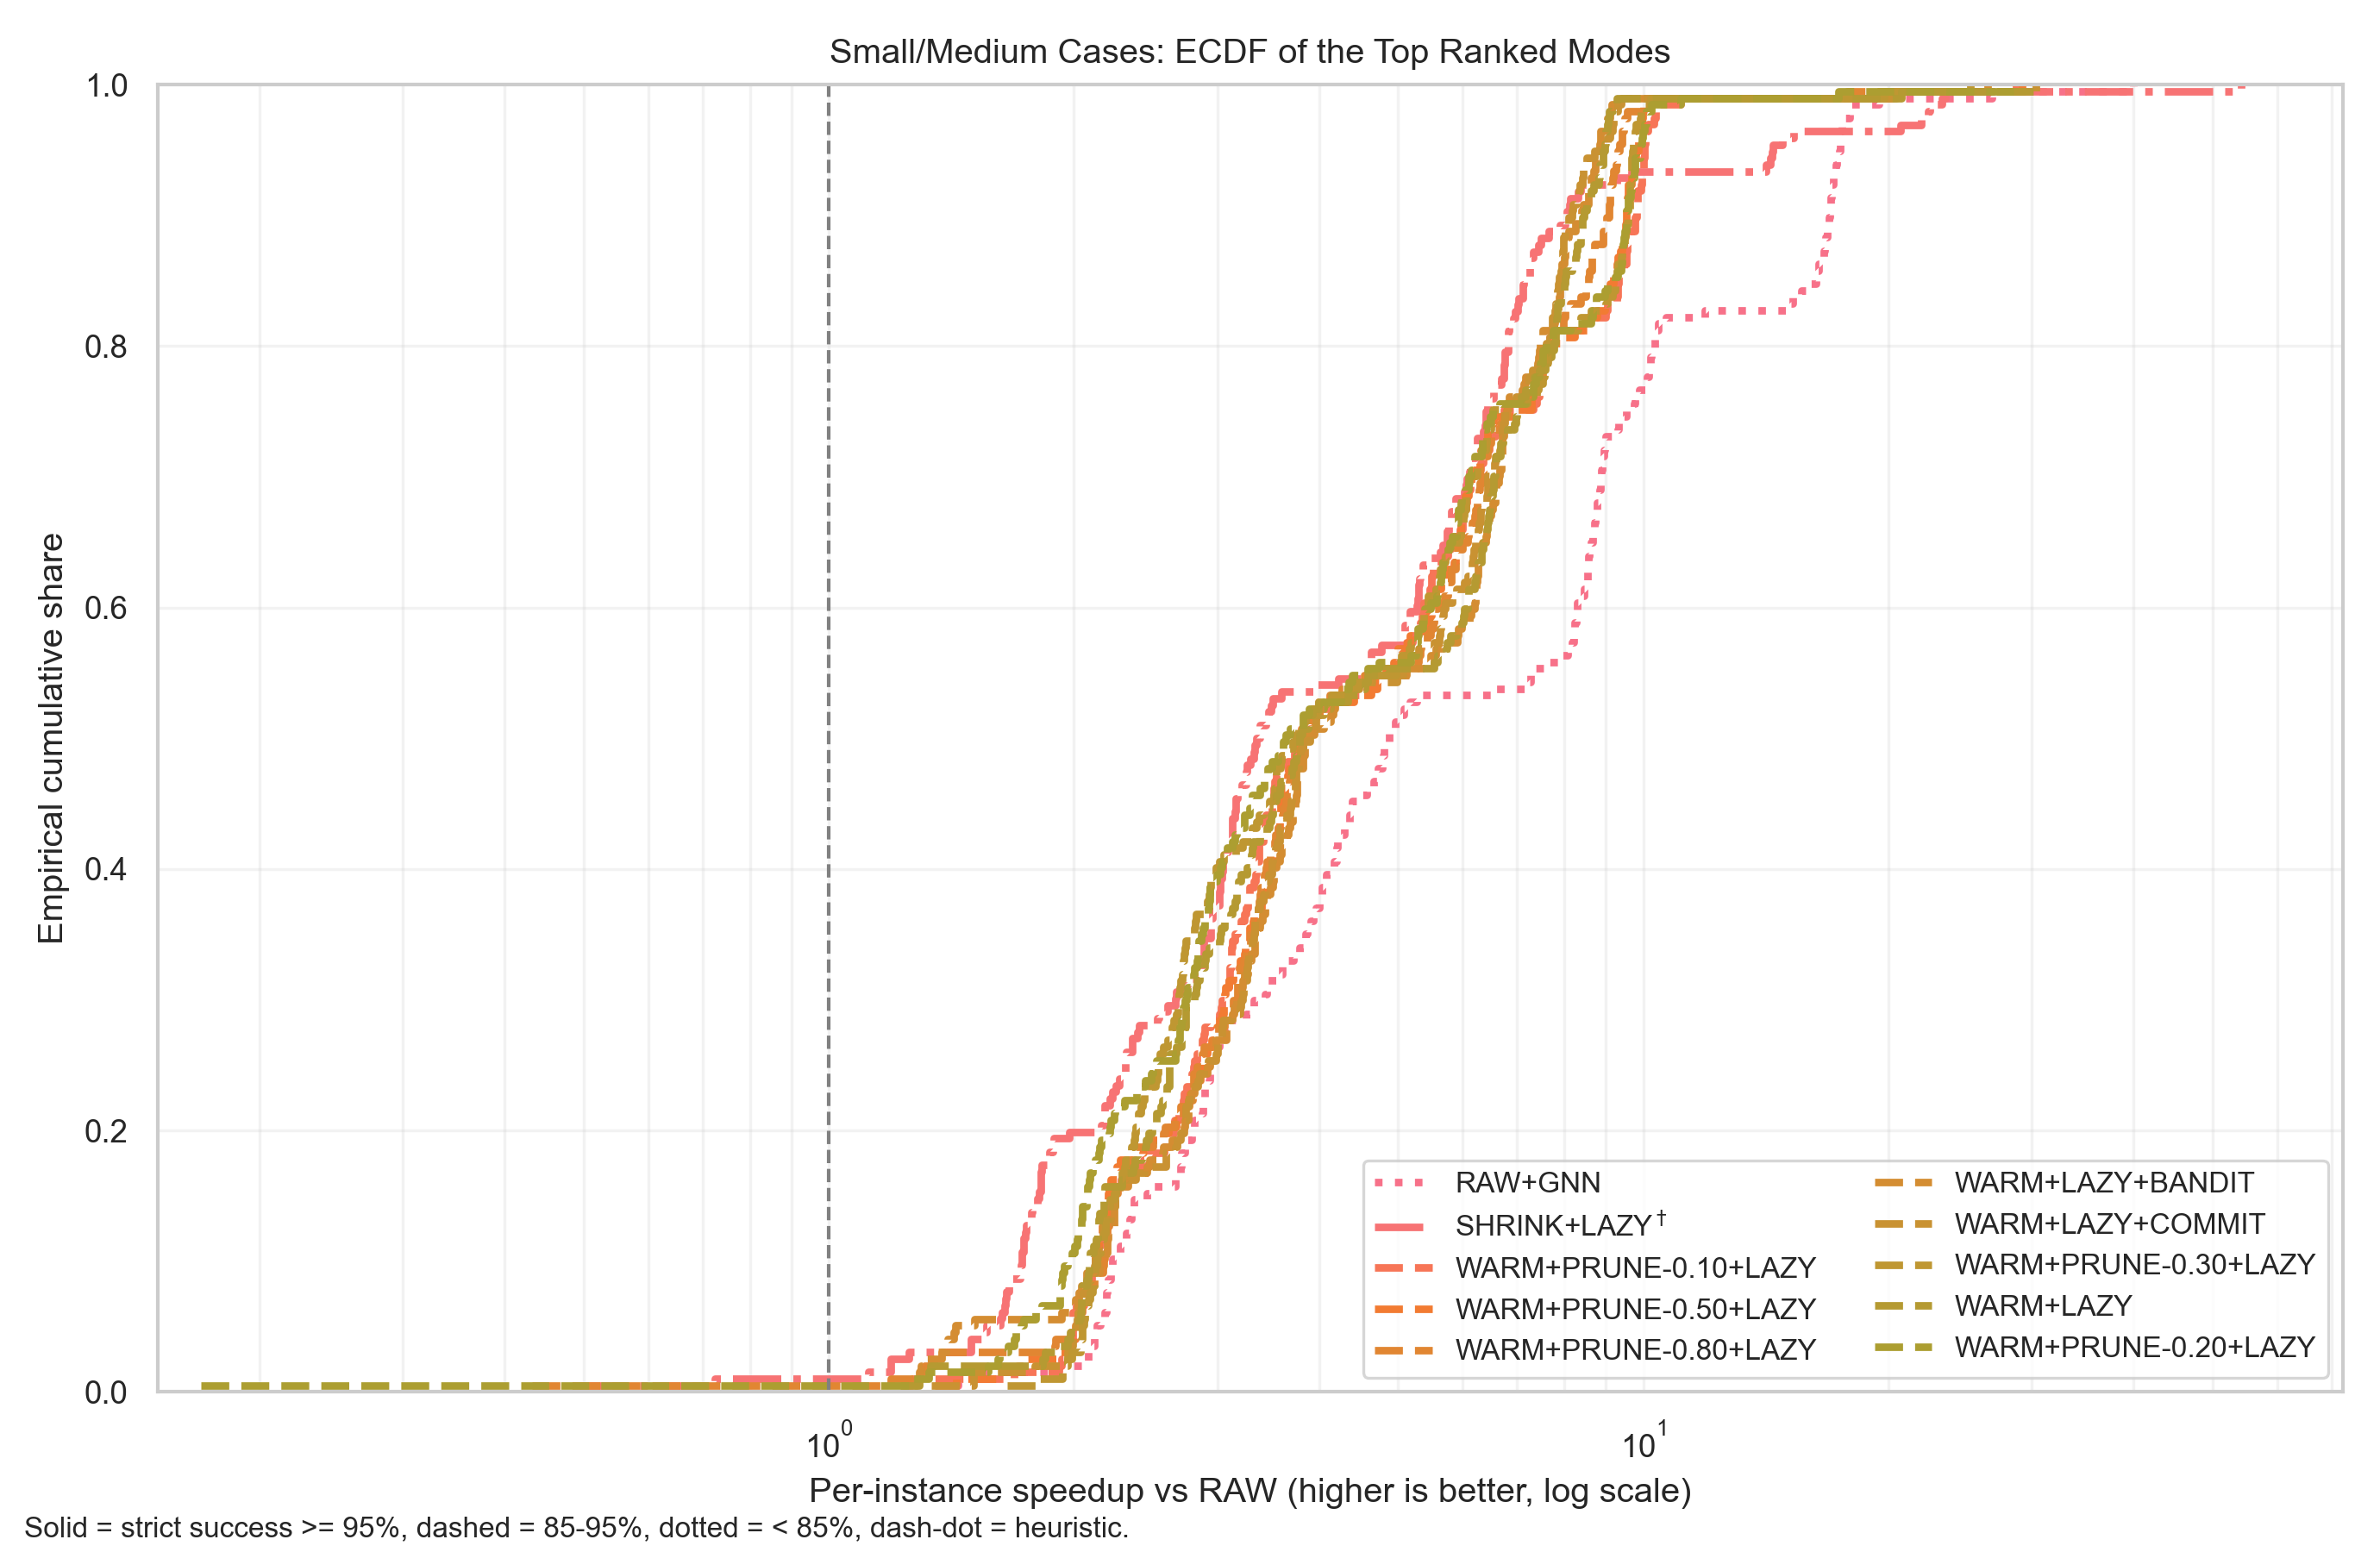
\includegraphics[width=\linewidth]{figures/ecdf.png}
  \caption{ECDF of relative speedup.}
  \label{fig:ecdf}
\end{figure*}

\begin{figure*}
  \centering
  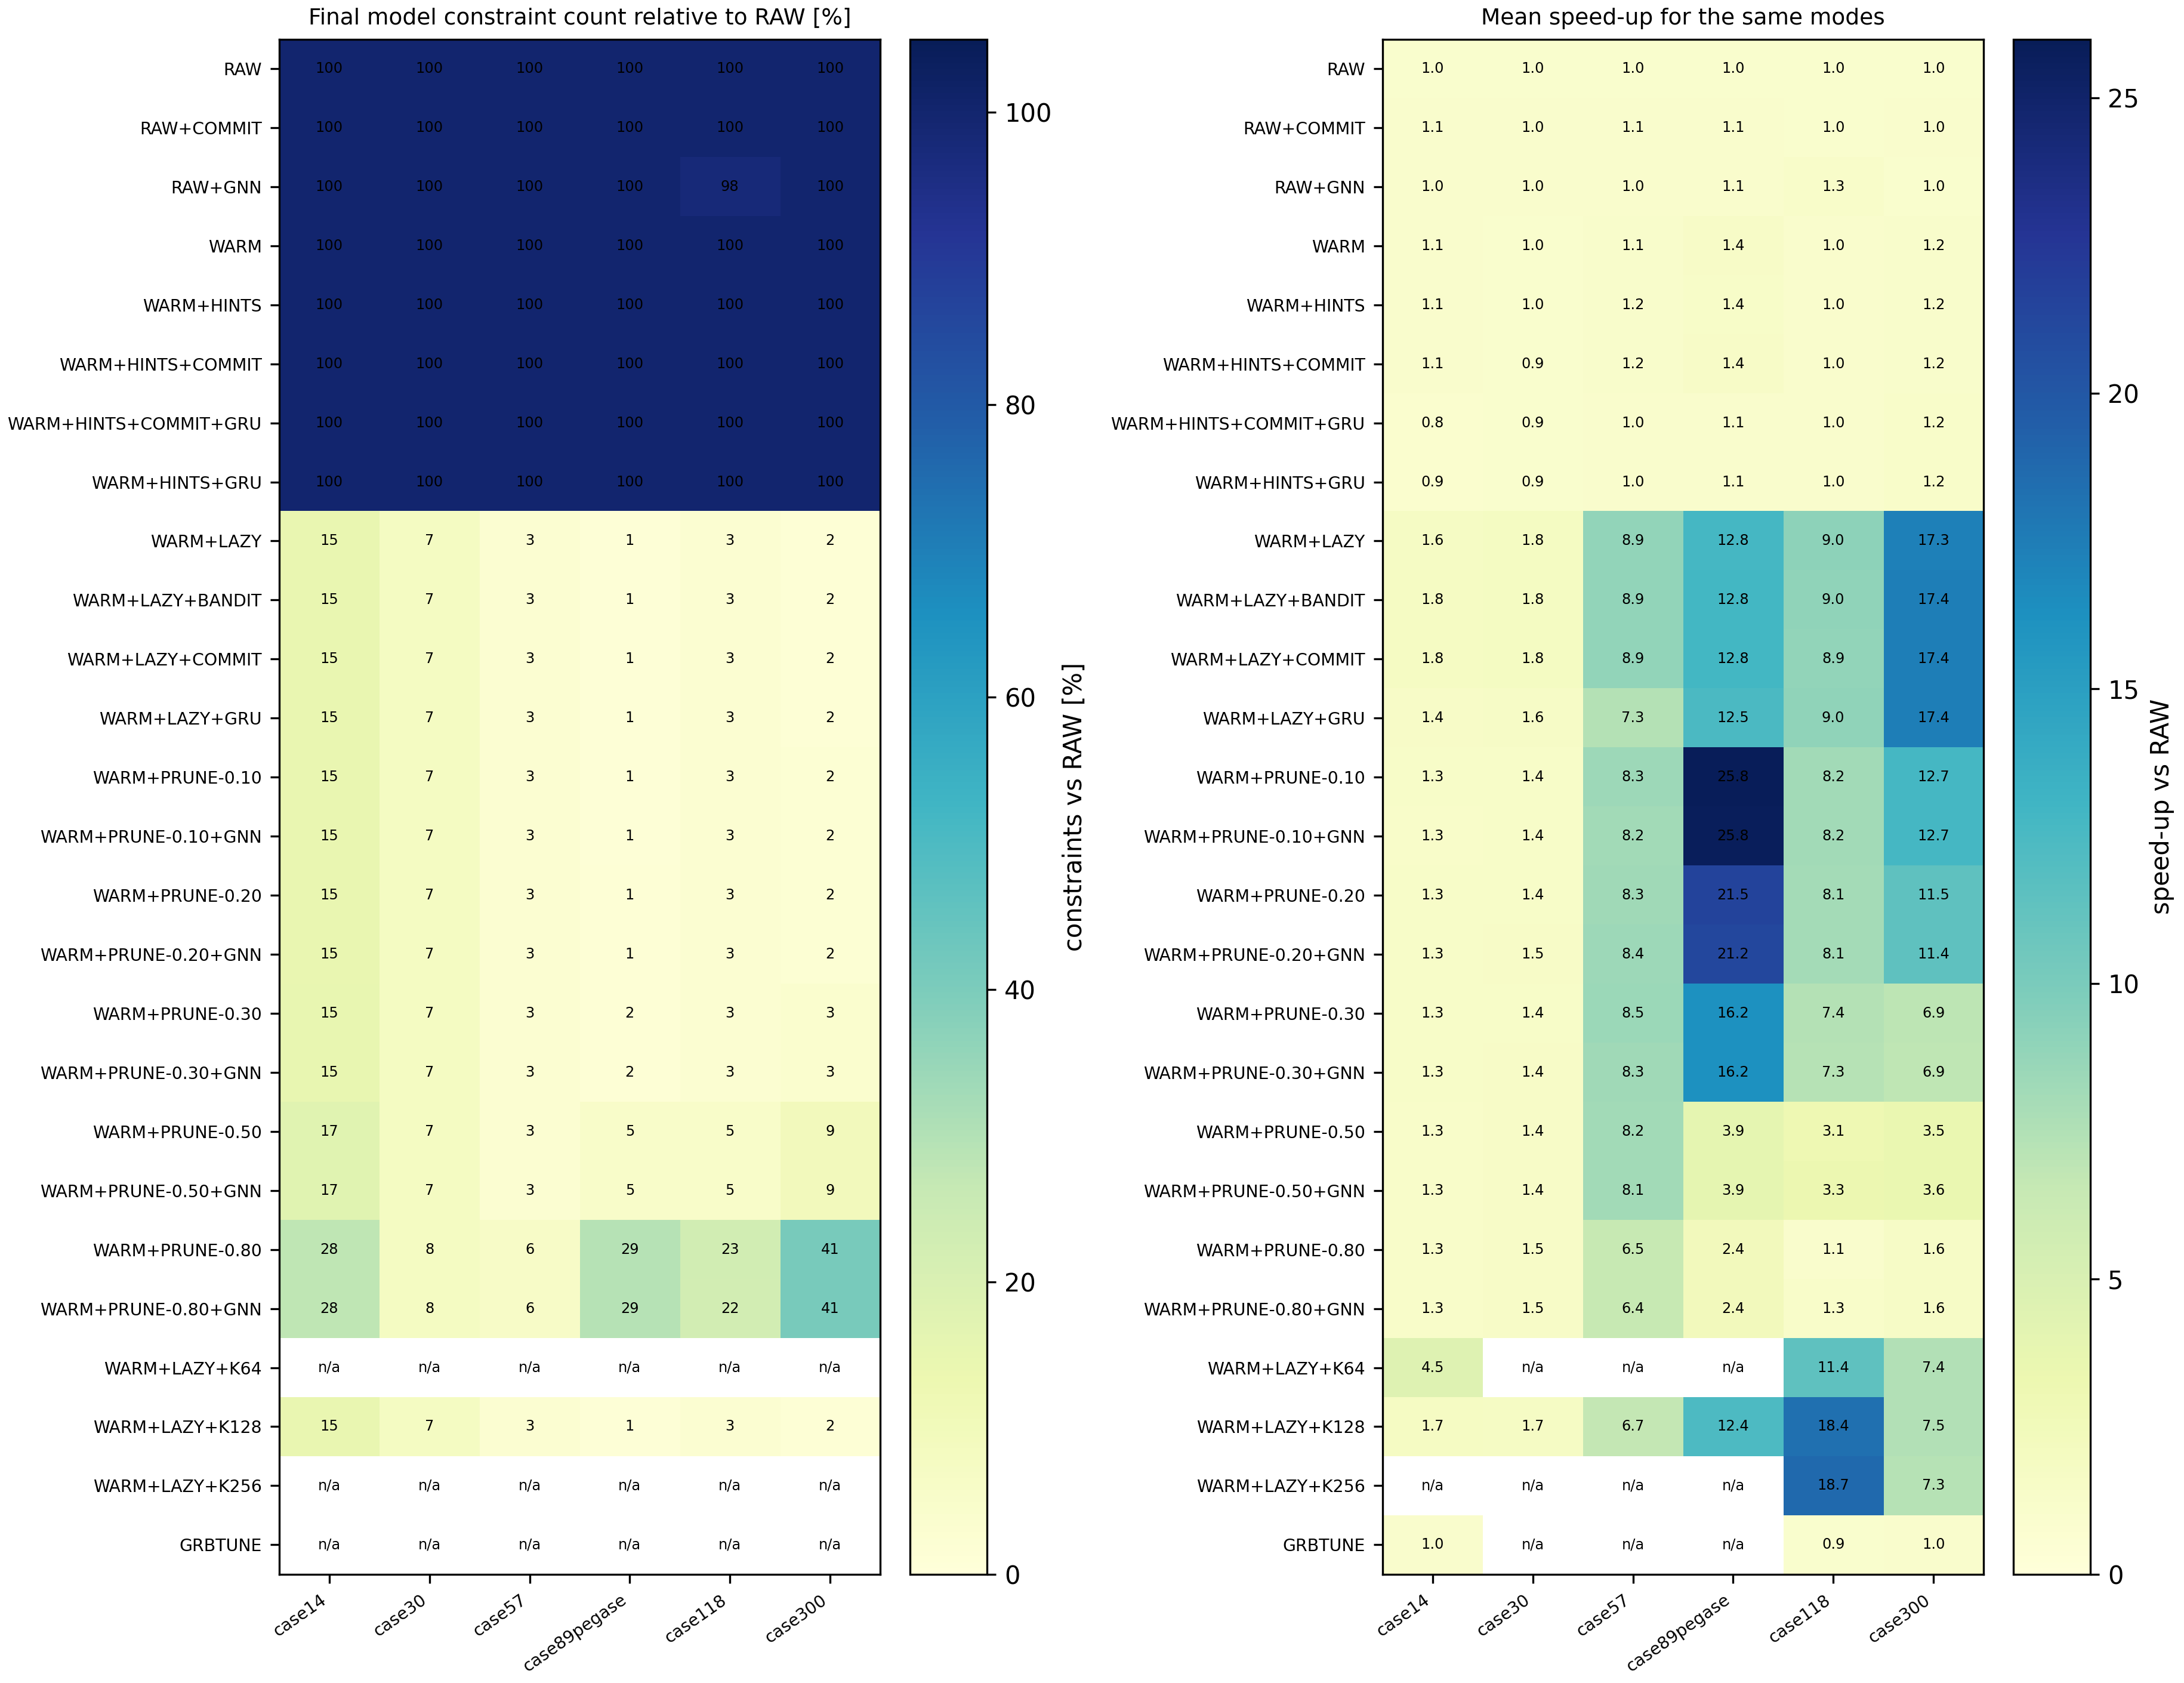
\includegraphics[width=\linewidth]{figures/constraint_reduction_speedup.png}
  \caption{Constraint reduction and speedup.}
  \label{fig:speedup_heatmap}
\end{figure*}

Experiments used Gurobi 12.1 on an AMD Ryzen 7840HS with 32 GB RAM. The benchmark contains six UnitCommitment MATPOWER cases~\cite{Xavier2024,MATPOWER,PEGASE}: 14, 30, 57, 89pegase, 118, and 300 buses. Each was converted into a multi-period DC-SCUC with full N-1 transmission security. A representative grbtune check on RAW case14, case118, and case300 isolates solver-parameter effects.

All modes share the same formulation, penalties, objective, and feasibility definitions. RAW is the full explicit N-1 model without starts or branching hints. WARM, HINTS, COMMIT, GRU, PRUNE, LAZY, and BANDIT are layered on RAW in controlled combinations.

Learning components use fixed train, validation, and test pools generated per case from dated UnitCommitment instances. The pools are then expanded by solver mode, so solver-run counts are larger than the number of unique calendar instances. Only test results are reported. Speedups are relative to paired RAW runs. We use ECDFs, bootstrap 95\% confidence intervals, and paired Wilcoxon signed-rank tests. The main CI table is Tab.~\ref{tab:speedup_ci}.

Each incumbent was audited against all base-case and post-contingency limits, including constraints removed by screening or not yet added by lazy callbacks. A run was N-1 feasible only if all audited violations were below $\varepsilon_{\mathrm{feas}}=10^{-6}$ MW. Failed audits, missing incumbents, and dates infeasible for all modes were excluded from speedup ratios. This full audit is needed because reduced models can omit active contingencies.

Because each benchmark requires a full MILP solve, learning components use one fixed split rather than $k$-fold cross-validation. The reported learning effects are split-specific, and seed sensitivity remains future work. Case14 and case30 are correctness checks because RAW runtimes are below one second. Practical claims rely mainly on case89pegase, case118, and case300. The case1354pegase experiment is a scalability stress test.


We performed 8,845 completed test solver runs over 360 test instances. These runs totaled 150.0 wall-clock hours and 94.3 solver-runtime hours. Overall, 93.9\% ended with an optimal solution, 4.6\% were infeasible, and 1.4\% hit the time limit. Training and preparation required 434 additional runs over 288 instances, adding 62.8 wall-clock hours and 51.9 solver-runtime hours. Reported online speedups exclude this preparation cost and assume amortization over repeated solves. At instance level, 95.6\% of unique test instances were solved optimally at least once. Cases 14--89pegase used 60 seconds. Larger cases used 600 seconds. Training and validation sets were solved separately.

Baseline methods are less robust on larger systems: RAW+COMMIT solves only 71\% of case300 instances optimally. For case57, the repeated 77/23/0 pattern reflects the same 14 infeasible dates across all 23 modes. This points to structural infeasibility rather than screening or warm-start failure. Those dates are excluded from speedup statistics. Aggressive pruning can also reduce case300 robustness.

Thus PRUNE-0.10 is the recommended screening default.

If all modes report infeasibility on the same date, we attribute it to the benchmark data or security requirement. If only an accelerated reduced model fails the audit while RAW or full LAZY succeeds, we attribute it to the acceleration policy. This prevents reduced-model optimality from being mistaken for secure feasibility.

\begin{table}[t]\centering
\caption{Representative speedups over RAW.}
\label{tab:main_results}
\footnotesize
\setlength{\tabcolsep}{3pt}
\resizebox{\linewidth}{!}{%
\begin{tabular}{|l|r|r|r|}
\hline
\textbf{Mode} & \textbf{Mean} & \textbf{Best mean} & \textbf{Opt. status} \\
\hline
RAW & 1.00x & 1.00x & 91\% \\
WARM & 1.14x & 1.43x & 93\% \\
WARM+LAZY & 8.59x & 17.35x & 96\% \\
WARM+LAZY+BANDIT & 8.61x & 17.38x & 96\% \\
WARM+PRUNE-0.10 & 9.64x & 25.83x & 96\% \\
WARM+PRUNE-0.50 & 3.56x & 8.16x & 96\% \\
GRBTUNE & 1.00x & 1.05x & 100\% \\
\hline
\end{tabular}
}
\end{table}

The RAW row in Tab.~\ref{tab:main_results} has a lower optimality rate because the full explicit N-1 model is the hardest formulation. Speedup ratios use only paired runs with feasible incumbents.

% \begin{table}[t]\centering
\caption{Status and audit pass rates. TL is time limit; no inc. means no incumbent; audit OK is audited N-1 feasible.}
\label{tab:audit_pass_rate}
\scriptsize
\setlength{\tabcolsep}{3pt}
\resizebox{\linewidth}{!}{%
\begin{tabular}{|l|r|r|r|r|r|}
\hline
\textbf{Mode} & \textbf{Opt.} & \textbf{TL} & \textbf{No inc.} & \textbf{Audit fail} & \textbf{Audit OK} \\
\hline
RAW & 91\% & 5\% & 4\% & 0\% & 91\% \\
WARM+LAZY & 96\% & 0\% & 4\% & 0\% & 96\% \\
WARM+LAZY+BANDIT & 96\% & 0\% & 4\% & 0\% & 96\% \\
WARM+PRUNE-0.10 & 96\% & 0\% & 4\% & 0\% & 96\% \\
WARM+LAZY+K128 & 96\% & 0\% & 4\% & 23\% & 73\% \\
\hline
\end{tabular}
}
\end{table}


% Tab.~\ref{tab:audit_pass_rate} separates reduced-model status from the post-solve audit; speedups are interpreted only on audited feasible runs.

\begin{sidewaystable*}\centering
\caption{Speedup factors with bootstrap 95\% confidence intervals (mean [CI\textsubscript{lo}, CI\textsubscript{hi}]).}
\label{tab:speedup_ci}
\renewcommand{\arraystretch}{1.2}
\footnotesize
\begin{tabular}{|l||c|c|c|c|c|c|}\hline
\textbf{Mode} & \textbf{case14} & \textbf{case30} & \textbf{case57} & \textbf{case89pegase} & \textbf{case118} & \textbf{case300} \\ \hline \hline
RAW+COMMIT & 1.06 [1.02, 1.12] & 1.03 [1.00, 1.07] & 1.06 [1.04, 1.09] & 1.09 [1.05, 1.14] & 1.01 [0.96, 1.04] & 1.02 [0.98, 1.05] \\ \hline
WARM & 1.06 [1.01, 1.12] & 0.98 [0.93, 1.03] & 1.15 [1.11, 1.19] & 1.43 [1.35, 1.52] & 1.03 [1.00, 1.06] & 1.19 [1.12, 1.27] \\ \hline
WARM+HINTS+COMMIT & 1.07 [1.02, 1.13] & 0.95 [0.90, 0.99] & 1.19 [1.15, 1.23] & 1.43 [1.36, 1.52] & 1.02 [0.98, 1.05] & 1.19 [1.12, 1.27] \\ \hline
WARM+LAZY & 1.64 [1.57, 1.74] & 1.85 [1.75, 1.93] & 8.89 [7.51, 10.39] & 12.77 [12.22, 13.34] & 9.04 [8.59, 9.53] & 17.35 [15.38, 19.37] \\ \hline
WARM+LAZY+BANDIT & 1.77 [1.68, 1.87] & 1.83 [1.74, 1.91] & 8.86 [7.53, 10.29] & 12.82 [12.27, 13.41] & 9.03 [8.62, 9.47] & 17.38 [15.39, 19.39] \\ \hline
WARM+PRUNE-0.10 & 1.34 [1.28, 1.42] & 1.41 [1.31, 1.51] & 8.34 [7.05, 9.73] & 25.83 [24.40, 27.26] & 8.22 [7.68, 8.75] & 12.72 [10.95, 14.55] \\ \hline
WARM+PRUNE-0.10+GNN & 1.27 [1.20, 1.34] & 1.42 [1.32, 1.52] & 8.18 [7.04, 9.48] & 25.75 [24.36, 27.14] & 8.17 [7.66, 8.70] & 12.71 [10.96, 14.54] \\ \hline
WARM+PRUNE-0.30 & 1.33 [1.26, 1.40] & 1.41 [1.32, 1.50] & 8.50 [7.19, 9.94] & 16.22 [14.12, 18.30] & 7.37 [6.68, 8.09] & 6.91 [6.11, 7.69] \\ \hline
WARM+PRUNE-0.50 & 1.27 [1.20, 1.34] & 1.44 [1.35, 1.54] & 8.16 [6.91, 9.51] & 3.92 [3.50, 4.40] & 3.08 [2.70, 3.52] & 3.50 [3.15, 3.87] \\ \hline
WARM+PRUNE-0.80 & 1.30 [1.24, 1.35] & 1.45 [1.37, 1.54] & 6.50 [5.60, 7.43] & 2.43 [2.28, 2.59] & 1.05 [0.96, 1.14] & 1.61 [1.49, 1.75] \\ \hline
\end{tabular}
\end{sidewaystable*}


\begin{table}[t]\centering
\caption{Constraint-reduction summary.}
\label{tab:constraint_reduction_compact}
\footnotesize
\setlength{\tabcolsep}{3pt}
\resizebox{\linewidth}{!}{%
\begin{tabular}{|l|r|r|r|}
\hline
\textbf{Mode} & \textbf{Root rows} & \textbf{N-1 pruned} & \textbf{Lazy cuts} \\
\hline
RAW & 100.0\% & -- & -- \\
WARM & 100.0\% & -- & -- \\
WARM+LAZY & 5.0\% & -- & 9{,}863 \\
WARM+LAZY+BANDIT & 5.0\% & -- & 721 \\
WARM+PRUNE-0.10 & 5.0\% & 99.95\% & -- \\
WARM+PRUNE-0.50 & 7.9\% & 97.00\% & -- \\
\hline
\end{tabular}
}
\end{table}

The first two percentage columns in Tab.~\ref{tab:constraint_reduction_compact} have different denominators. ``Root rows'' is the initial/root row count before lazy cuts as a share of RAW rows. ``N-1 pruned'' is the fraction of candidate post-contingency rows removed before optimization. Lazy cuts are added after the root model through callbacks.

Tabs.~\ref{tab:main_results}--\ref{tab:speedup_ci} and Fig.~\ref{fig:speedup_heatmap} summarize speedups. The strongest accelerations come from empirically safe screening and lazy enforcement. WARM+PRUNE-0.10 has the highest mean speedup, 9.64x. WARM+LAZY+BANDIT reaches 8.61x, only marginally above plain WARM+LAZY. Pruning is best on case89pegase (25.83x, 95\% CI $[24.40, 27.26]$). Lazy enforcement is best on case300 (17.38x, 95\% CI $[15.39, 19.39]$). These gains follow the root-model reductions in Tab.~\ref{tab:constraint_reduction_compact}. Thus N-1 constraint management drives the speedups.

RAW and WARM expose the full N-1 model at the root, so warm starts mainly affect incumbent discovery. LAZY and PRUNE shrink the root relaxation to about 5\% of RAW rows. Plain LAZY adds about 9{,}863 callback cuts on average. BANDIT adds about 721 with almost no extra speedup.

Solver-native starts help branch-and-bound heuristics, but they do not remove the transmission rows that dominate the root relaxation. Screening and lazy enforcement attack this N-1 burden directly.

The ablations are mostly negative. GNN speedups stay close to 1-NN (ratios 0.987--1.035). Fixed-$K$ lazy cuts can be fast on case118, but on case300 they are slower than LAZY/BANDIT and pass the audit in only 66\% of runs. Gurobi tuning gives only 0.93x on case118 and 1.02x on case300.

These negative results rule out simple explanations based on model complexity or generic parameter tuning.

Acceleration quality cannot be judged by reduced-model runtime alone. A smaller model may solve quickly but still fail the full N-1 audit. We therefore prioritize audited feasible speedup over reduced-model solver status.

Fig.~\ref{fig:ecdf} shows consistent gains from PRUNE-0.10 and the largest difficult-instance gains from lazy enforcement, with many runs above 10x speedup. Wilcoxon tests confirm WARM + PRUNE-0.10, WARM + LAZY, and WARM + LAZY + BANDIT against RAW on every case ($p<10^{-7}$).

Solver-runtime medians show the same trend. Case118 drops from 40.46s to 4.40s with WARM+LAZY+BANDIT. Case300 drops from 199.22s to 13.82s.

The ECDF view shows why both mechanisms remain useful. PRUNE-0.10 gives predictable gains, while lazy enforcement gives the largest gains on the hardest instances.

For scalability, we used case1354pegase (1{,}354 buses, 260 generators, 1{,}991 branches, 1{,}288 contingencies, 36 periods) from MATPOWER/PEGASE~\cite{MATPOWER,PEGASE} as a feasibility stress test. MATPOWER describes these data as fictitious and for algorithm validation rather than operation or planning. The model without contingencies has 317{,}484 rows. Static N-1 enforcement would add $52{,}218{,}216$ candidate post-contingency rows in this implementation: two-sided emergency limits for monitored line- and generator-contingency pairs after invalid outage/self-monitoring pairs and out-of-service elements are excluded across all 36 periods. All stress-test runs use lazy enforcement. Table~\ref{tab:case1354} reports one representative held-out instance. The larger campaign also included 24 training days and two held-out test days, giving 74 training/preparation runs and 66 test-mode runs.

\begin{table}[t]\centering
\caption{case1354pegase stress-test results.}
\label{tab:case1354}
\small
\begin{tabular}{|l|l|l|r|r|l|}
\hline
\textbf{Mode} & \textbf{Status} & \textbf{Time [s]} & \textbf{Gap} & \textbf{Obj.} & \textbf{Audit} \\
\hline
        WARM & TL & 602 & --- & --- & --- \\
        LAZY-All ($K{=}0$) & TL & 607 & 12.3\% & $174.80$M & \checkmark \\
        LAZY-K64 & OPT & 247 & 4.6\% & $108.32$M & small viol. \\
        LAZY-K128 & TL & 600 & --- & --- & --- \\
        LAZY-BANDIT & OPT & 266 & 5.0\% & $108.92$M & small viol. \\
        LAZY+COMMIT & TL & 601 & 8.2\% & $166.95$M & \checkmark \\
        LAZY+GRU & TL & 600 & 11.4\% & $172.77$M & \checkmark \\
\hline
\end{tabular}
\end{table}


The WARM reference run finds no feasible integer solution within the budget, so no post-solve N-1 audit can be applied to that row.

LAZY-All ($K{=}0$) finds an N-1-feasible solution with a 12.3\% MIP gap because every detected violation is added. LAZY+COMMIT gives the best audited feasible objective at 8.2\% gap, and LAZY+GRU reaches 11.4\%. These results suggest useful learning cues, but they are not general robustness evidence.

Fixed-$K$ and BANDIT solve faster by adding fewer cuts, but they do not guarantee closure of all N-1 constraints. OPT means optimality of the reduced callback model. Full N-1 validity is decided by the audit. LAZY-K64 and LAZY-BANDIT reach OPT faster but leave small residual violations. Thus lazy constraints produce audited feasible solutions on a system roughly four times larger than the main benchmark. The stress test should be read with caution. It shows that the constraint-management logic remains operational when static N-1 enforcement is no longer practical. It does not prove large-scale robustness.

\section{Conclusion}

This study shows that constraint management is the most effective accelerator among the tested methods. The key is to reduce or delay post-contingency constraints while keeping the full post-solve feasibility audit. We tested 360 MATPOWER instances and 8,845 completed runs with Gurobi 12.1 on a Ryzen 7840HS/32GB system. Two strategies gave the largest and most consistent gains. The first is screening redundant contingencies before solving. It uses simple data-driven predictors and LODF/PTDF sensitivities. The second is generating only the necessary contingency constraints on demand during branch-and-bound.

The recommended screening threshold preserved audited feasibility on the reported benchmark runs, and lazy generation often achieved the best performance on the hardest individual instances. In aggregate, the strongest screening threshold produced the highest average speedup (approximately $9.6\times$ over a fully explicit baseline), while lazy generation dominated the largest case in the benchmark. The revision analysis also shows that these gains coincide with very large reductions in explicit contingency constraints, typically above 99.7\% on the larger systems, and are statistically significant on every benchmark case (paired Wilcoxon $p<10^{-7}$).

Learning signals applied to the discrete search, including warm starts from historical solutions, lightweight initializers, and branching guidance based on commitment probability, yielded smaller average speedups (around $1.1\times$). In our benchmark, the GNN screener did not consistently outperform the simpler 1-NN baseline, the GRU initializer was unstable on smaller cases, and the adaptive BANDIT policy improved only marginally over plain LAZY. These observations support a ``constraint-economy first'' design: shrink or postpone the contingency set, verify security with a full N-1 audit, and only then add inexpensive learning cues to guide the search.

\begin{thebibliography}{99}

\bibitem{Merlin1983}
A.~Merlin and P.~Sandrin, ``A new method for unit commitment at Electricit\'e de France,'' \emph{IEEE Trans. Power Appar. Syst.}, vol.~PAS-102, no.~5, pp.~1218--1225, May 1983, doi: 10.1109/TPAS.1983.318063.

\bibitem{Carrion2006}
M.~Carri\'on and J.~M. Arroyo, ``A computationally efficient mixed-integer linear formulation for the thermal unit commitment problem,'' \emph{IEEE Trans. Power Syst.}, vol.~21, no.~3, pp.~1371--1378, Aug. 2006, doi: 10.1109/TPWRS.2006.876672.

\bibitem{Ostrowski2012}
J.~Ostrowski, M.~F. Anjos, and A.~Vannelli, ``Tight mixed-integer linear programming formulations for the unit commitment problem,'' \emph{IEEE Trans. Power Syst.}, vol.~27, no.~1, pp.~39--46, Feb. 2012, doi: 10.1109/TPWRS.2011.2162008.

\bibitem{Morales2013}
J.~M. Morales, A.~J. Conejo, H.~Madsen, P.~Pinson, and M.~Zugno, \emph{Integrating Renewables in Electricity Markets: Operational Problems}. Boston, MA, USA: Springer, 2014, doi: 10.1007/978-1-4614-9411-9.

\bibitem{Christie2000}
R.~D. Christie, B.~F. Wollenberg, and I.~Wangensteen, ``Transmission management in the deregulated environment,'' \emph{Proc. IEEE}, vol.~88, no.~2, pp.~170--195, Feb. 2000, doi: 10.1109/5.823997.

\bibitem{Tejada2018}
D.~A. Tejada-Arango, P.~S\'anchez-Mart\'in, and A.~Ramos, ``Security constrained unit commitment using line outage distribution factors,'' \emph{IEEE Trans. Power Syst.}, vol.~33, no.~1, pp.~329--337, Jan. 2018, doi: 10.1109/TPWRS.2017.2686701.

\bibitem{Holzer2024}
J.~T. Holzer, Y.~Chen, Z.~Wu, F.~Pan, and A.~Veeramany, ``Fast simultaneous feasibility test for security constrained unit commitment,'' \emph{IEEE Trans. Power Syst.}, vol.~39, no.~1, pp.~1068--1078, Jan. 2024, doi: 10.1109/TPWRS.2023.3265269.

\bibitem{Bengio2021}
Y.~Bengio, A.~Lodi, and A.~Prouvost, ``Machine learning for combinatorial optimization: A methodological tour d'horizon,'' \emph{European J. Oper. Res.}, vol.~290, no.~2, pp.~405--421, Apr. 2021, doi: 10.1016/j.ejor.2020.07.063.

\bibitem{Xavier2019}
A.~S. Xavier, F.~Qiu, and S.~Ahmed, ``Learning to solve large-scale security-constrained unit commitment problems,'' \emph{INFORMS J. Comput.}, vol.~33, no.~2, pp.~739--756, May 2021, doi: 10.1287/ijoc.2020.0976.

\bibitem{Quarm2021}
E.~Quarm Jnr. and R.~Madani, ``Scalable security-constrained unit commitment under uncertainty via cone programming relaxation,'' \emph{IEEE Trans. Power Syst.}, vol.~36, no.~5, pp.~4733--4744, Sept. 2021, doi: 10.1109/TPWRS.2021.3062203.

\bibitem{Donti2021}
P.~L. Donti, D.~Rolnick, and J.~Z. Kolter, ``DC3: A learning method for optimization with hard constraints,'' in \emph{Proc. Int. Conf. Learn. Represent. (ICLR)}, 2021, arXiv:2104.12225, doi: 10.48550/arXiv.2104.12225.

\bibitem{JimenezCordero2022}
A.~Jim\'enez-Cordero, J.~M. Morales, and S.~Pineda, ``Warm-starting constraint generation for mixed-integer optimization: A machine learning approach,'' \emph{Knowledge-Based Systems}, vol.~253, Art.~no.~109570, Oct. 2022, doi: 10.1016/j.knosys.2022.109570.

\bibitem{Hamilton2017}
W.~L. Hamilton, R.~Ying, and J.~Leskovec, ``Inductive representation learning on large graphs,'' in \emph{NeurIPS}, 2017.

\bibitem{Prokhorenkova2018}
L.~Prokhorenkova \emph{et al.}, ``CatBoost: unbiased boosting with categorical features,'' in \emph{NeurIPS}, 2018.

\bibitem{GurobiLazy}
Gurobi Optimization, LLC, ``Gurobi Optimizer Reference Manual: LazyConstraints parameter,'' 2026.

\bibitem{Xavier2024}
A.~S. Xavier, A.~M. Kazachkov, O.~Yurdakul, J.~He, and F.~Qiu, ``UnitCommitment.jl: A Julia/JuMP optimization package for security-constrained unit commitment (Version 0.4),'' Zenodo, 2024, doi: 10.5281/zenodo.4269874.

\bibitem{MATPOWER}
R.~D. Zimmerman, C.~E. Murillo-S\'anchez, and R.~J. Thomas, ``MATPOWER: steady-state operations, planning, and analysis tools for power systems research and education,'' \emph{IEEE Trans. Power Syst.}, 2011.

\bibitem{PEGASE}
C.~Josz, S.~Fliscounakis, J.~Maeght, and P.~Panciatici, ``AC power flow data in MATPOWER and QCQP format: iTesla, RTE snapshots, and PEGASE,'' arXiv:1603.01533, 2016.

\end{thebibliography}

\end{document}
